% \documentclass{beamer}
\documentclass[aspectratio=141]{beamer}
\usepackage[utf8]{inputenc}
\usepackage[T1]{fontenc}

\usepackage{fontawesome}
\usepackage[outline]{contour}
\usepackage{hyperref}
\usepackage[backend=biber]{biblatex}
\usepackage{tabularx}
\usepackage{multirow}
\usepackage{booktabs}
\usepackage{nicematrix}

\addbibresource{my_biblio.bib}

\title[Approaches for Domain Adaptive Object Detection in Production Environments]{Approaches for Domain Adaptive Object Detection in Production Environments}
\date[04/04/2022]{April 4, 2022}
\author[G. Degola]{Gabriele~\textsc{Degola}}

\newcommand\pro{\item[\faThumbsOUp]}
\newcommand\con{\item[\faThumbsODown]}

\newcommand{\quotes}[1]{``#1''}

\usetheme{DE}

\setbeamertemplate{footline}[my footline]

\AtBeginSection[]
{
  \begin{frame}
    \frametitle{Contents}
    \tableofcontents[currentsection]
  \end{frame}
}

\begin{document}

\begin{frame}
\titlepage
\end{frame}

\begin{frame}
    \frametitle{Contents}
    \tableofcontents
\end{frame}

\section{Introduction}

\begin{frame}{Introduction}
    \framesubtitle{Introduction}
    
    \begin{overlayarea}{\textwidth}{6cm}
    \begin{itemize}
        \pro<1-> \alert{Deep learning} methods are extremely effective on \alert{computer vision} tasks
        \only<1>{
            \begin{center}
            	\item[]
            	\hspace{-.06\textwidth}
                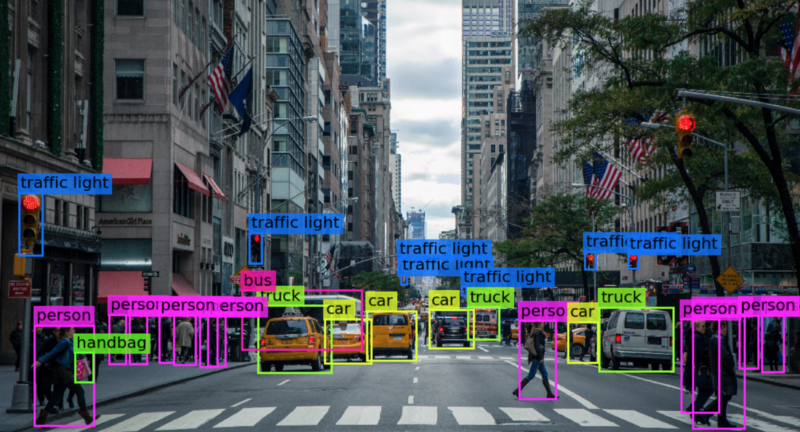
\includegraphics[width=.45\textwidth]{imgs/detection.png}
                \hspace{.01\textwidth}
                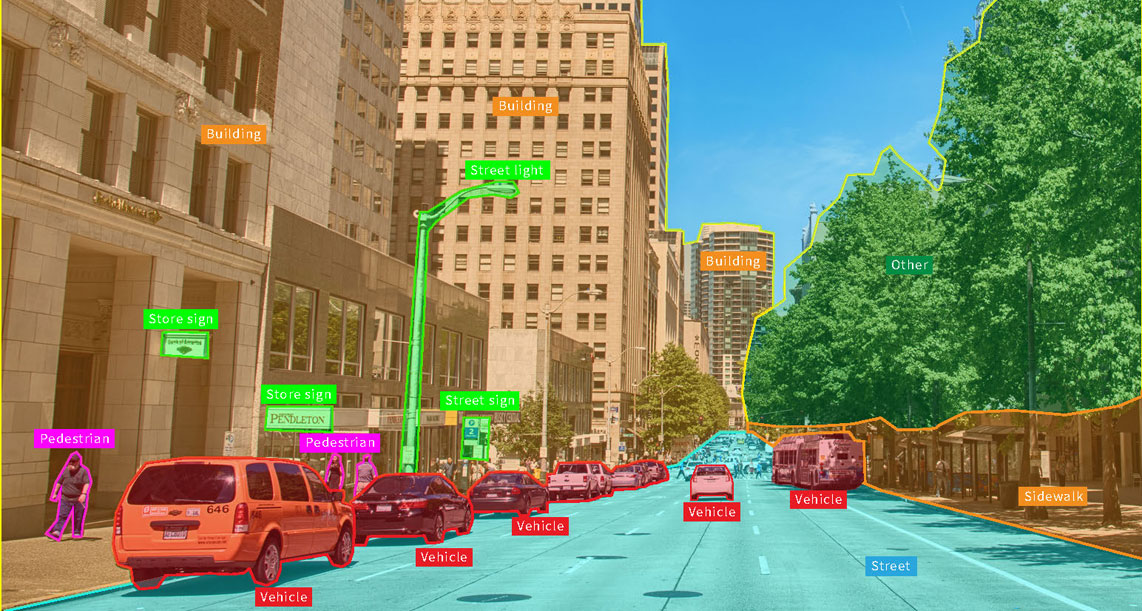
\includegraphics[width=.45\textwidth]{imgs/segmentation.png}
            \end{center}
        }
        \con<2-> ...but data collection and annotation is expensive and time-consuming
        \vspace*{3mm}
        \pro<3-> A solution is to use \alert{synthetic} data to simulate \alert{reality}
        \only<3>{
            \begin{center}
                \item[]
                \hspace{-.06\textwidth}
                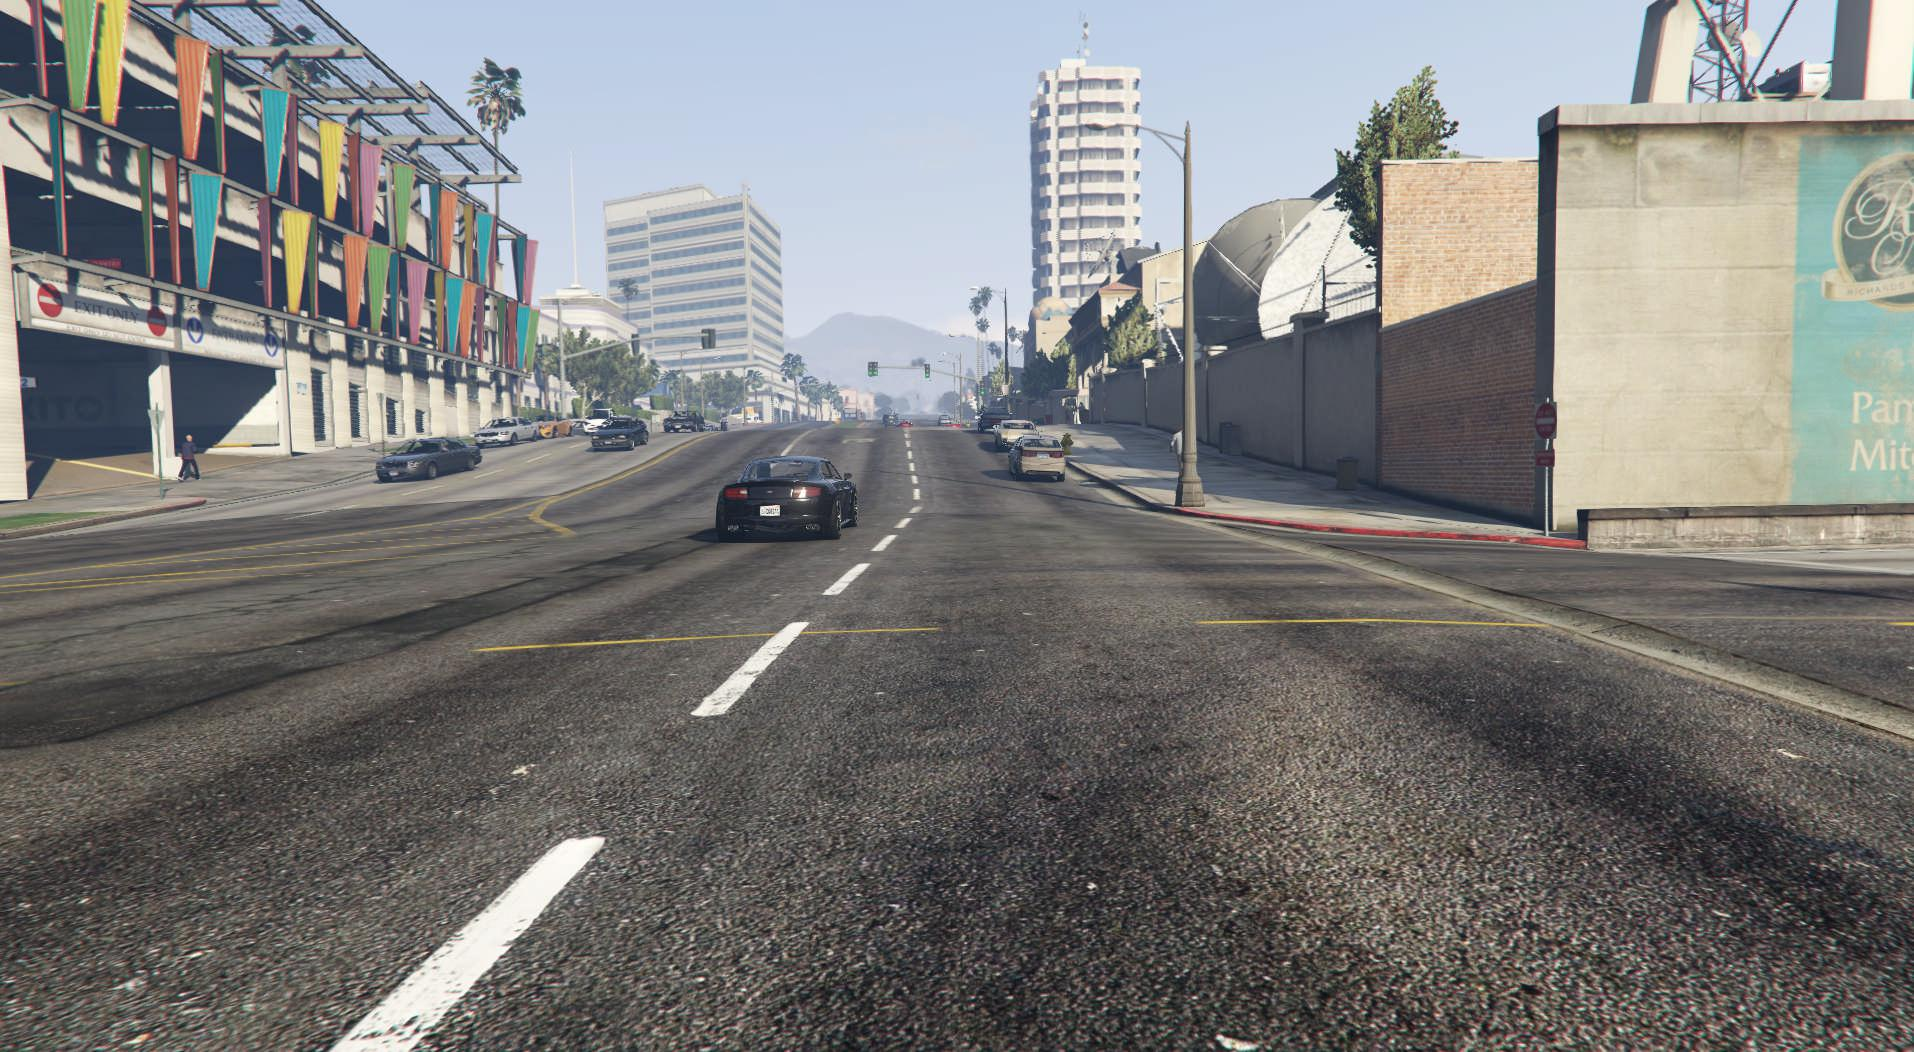
\includegraphics[width=.45\textwidth]{imgs/sim10k.jpg}
                \hspace{.01\textwidth}
                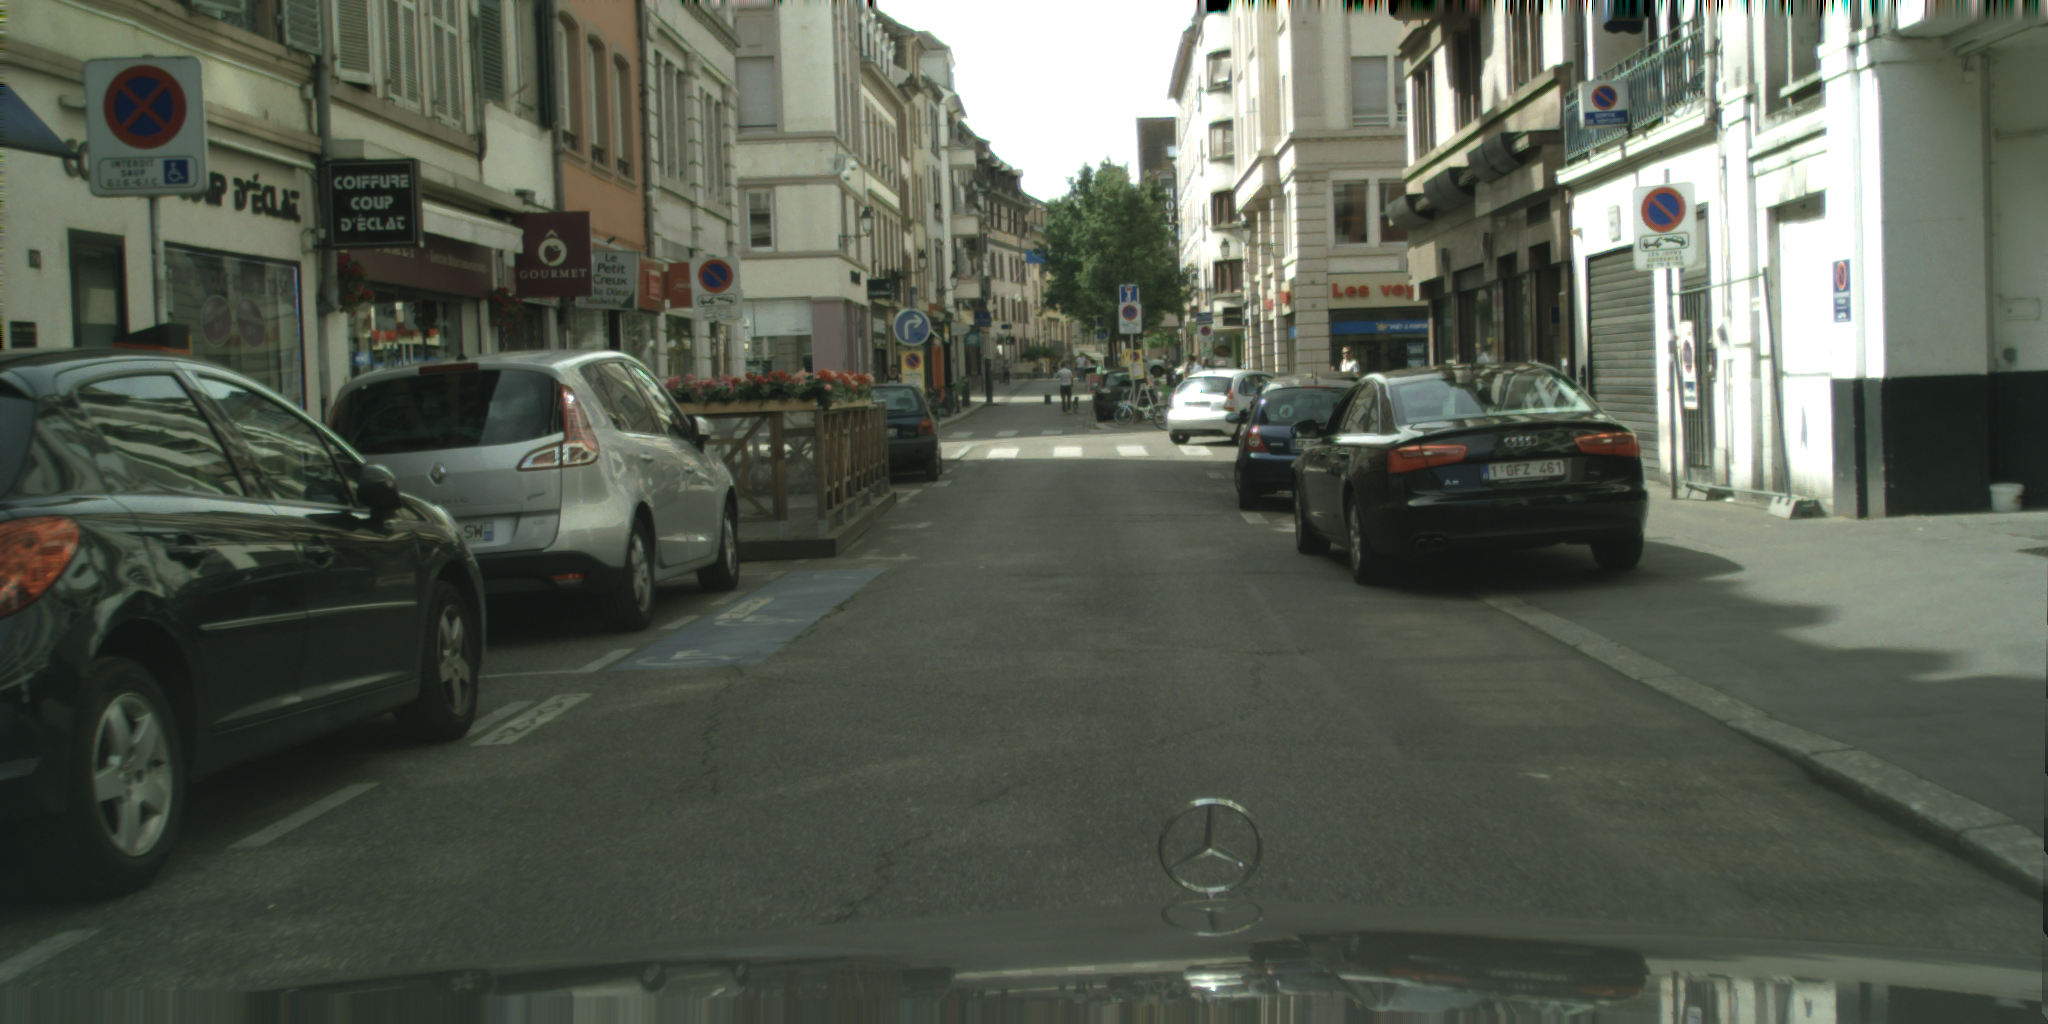
\includegraphics[width=.45\textwidth]{imgs/cityscapes.png}
            \end{center}
        }
        \con<4-> \textit{Machine learning} models expect \alert{training} and \alert{test} data to be drawn from the same \alert{data distribution}
        \vspace*{3mm}
        \pro<5-> \alert{\textbf{Domain adaptation}} methods transfer knowledge between domains
    \end{itemize}
    \end{overlayarea}
\end{frame}

\begin{frame}{Introduction}
    \framesubtitle{Context}
    
    \begin{itemize}
        %\item Six months internship, as part of Erasmus\texttt{+} double degree at \textit{Grenoble INP - Ensimag}
        \item Thesis conducted at \alert{Neovision}\footnote{\url{https://neovision.fr/en/}}, engineering company based in Grenoble, France, and specialized in artificial intelligence
        \vspace*{2mm}
        \begin{center}
            \fbox{
\includegraphics[width=.4\textwidth]{imgs/neovision.png}}
        \end{center}
        \vspace*{2mm}
        \begin{itemize}
            \item Lack of annotated data is a big obstacle for \textit{machine learning} projects
            \item Domain adaptation methods depend on specific network architectures, with deep modifications
        \end{itemize}
        \item[\contour{DEgreen}{$\Rightarrow$}] Domain adaptation can raise performances, but is complicated to set up in industrial projects
    \end{itemize}
\end{frame}

\begin{frame}{Introduction}
    \framesubtitle{Method}
    
    \begin{itemize}
    	\item Focus on \alert{object detection} task and transfer from synthetic to real images
    	\begin{itemize}
    		\item Synthetic dataset: \alert{\textit{Sim10k}}
    		\item Real dataset: \alert{\textit{CityScapes}}
    	\end{itemize}
    	\vspace*{4mm}
    	\item Research of \quotes{simple} approaches for domain adaptation
    	\begin{itemize}
    		\item Domain randomization through data augmentation
    		\item Matching image statistics between domains
    	\end{itemize}
	    \vspace*{4mm}
    	\item Analysis of popular domain adaptation methods and of their issues
    	\begin{itemize}
    	    \item Domain adaptation for one and two stage object detectors: Faster R-CNN\footfullcite{ren2016faster} and RetinaNet\footfullcite{lin2018focal}
    	\end{itemize}
    \end{itemize}
\end{frame}


\section{Domain adaptation}
\begin{frame}{Domain adaptation}
    \framesubtitle{Computer vision}
	\begin{itemize}
	\item \alert{Convolutional Neural Networks} (CNNs) extract features from images
	\item Three main tasks:
		\begin{itemize}
			\item \alert{Image classification}: class of an image
			\item \alert{Object detection}: position and class for all object in an image
			\item \alert{Semantic segmentation}: class of each pixel in an image
		\end{itemize}
	\end{itemize}
	
	\begin{center}
		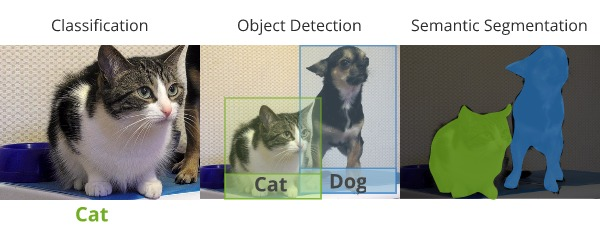
\includegraphics[width=.7\textwidth]{imgs/classdetseg.jpeg}
	\end{center}
\end{frame}

\begin{frame}{Domain adaptation}
    \framesubtitle{Domain adaptation}
    
	\begin{itemize}
	    \item Special case of \alert{transfer learning}
	    \vspace*{4mm}
	    \item Goal to transfer knowledge acquired on a \alert{source} domain (synthetic images) to a \alert{target} domain (real images), without training a new model from scratch
	    \vspace*{4mm}
		\item Source domain is annotated, while target domain is not: \alert{unsupervised} domain adaptation
	\end{itemize}
\end{frame}

\begin{frame}{Domain adaptation}
    \framesubtitle{Domain adaptation approaches}
    
    \begin{columns}
        \column{0.6\textwidth}
        \vspace*{-9mm}
        \begin{itemize}
            \item \textcolor<2->{gray}{
                \textbf{\textit{Domain invariant feature learning}}
                \begin{itemize}
                    \item \textcolor<2->{gray}{Goal of aligning feature distributions}
                    \item \textcolor<2->{gray}{After alignment, it is impossible to determine from which domain features are extracted}
                    \item \textcolor<2->{gray}{\textit{Adversarial} approach: feature extractor evolves with the aim of fooling a domain classifier}
                \end{itemize}
            }
            \vspace*{2mm}
            \item<2-> \textbf{\textit{Domain mapping}}
                \begin{itemize}
                    \item Images from source domain are transformed to look like the target domain
                    \item Annotations are not altered by the style transfer
                \end{itemize}
        \end{itemize}
        
        \column{0.4\textwidth}
        \only<1>{
            \begin{center}
                \vspace*{-10mm}
                \fbox{\parbox{.9\textwidth}{
                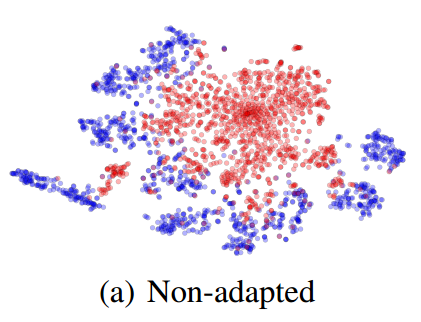
\includegraphics[width=\linewidth]{imgs/da_nonadapted.png}
                
                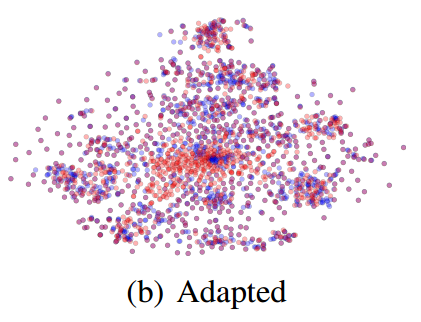
\includegraphics[width=\linewidth]{imgs/da_adapted.png}}}
            \end{center}
        }
        \only<2>{
            \begin{center}
                \vspace*{-7mm}
                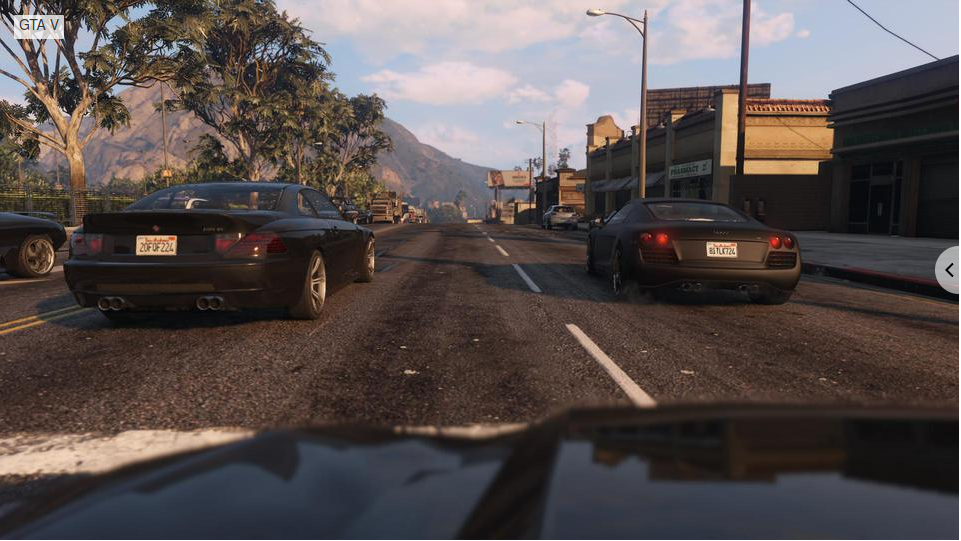
\includegraphics[width=\textwidth]{imgs/gta1.png}\\
                \vspace*{2mm}
                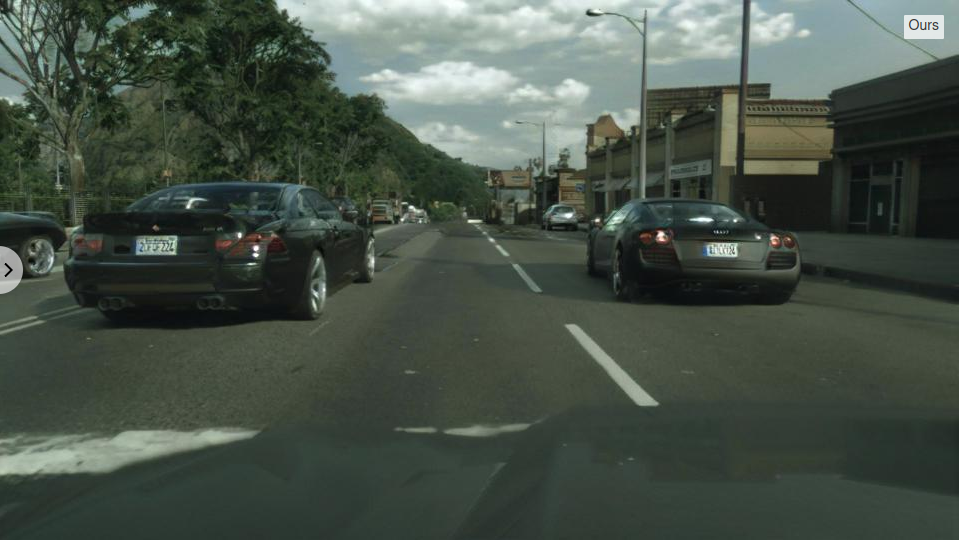
\includegraphics[width=\textwidth]{imgs/real1.png}
            \end{center}
        }
    \end{columns}
\end{frame}


\section{Method}

\begin{frame}{Method}
    \framesubtitle{Data augmentation for domain randomization}
    \begin{overlayarea}{\textwidth}{12cm}
    \begin{itemize}
        \item<1-> \alert{Data augmentation}:
        \begin{itemize}
            \item Standard technique to ease the training of deep neural networks
            \item Training images are randomly modified to introduce new data and increase variability
            \item Geometric or color-based
        \end{itemize}
        \only<1>{
            \begin{center}
                \item[]
                \hspace{-.06\textwidth}
                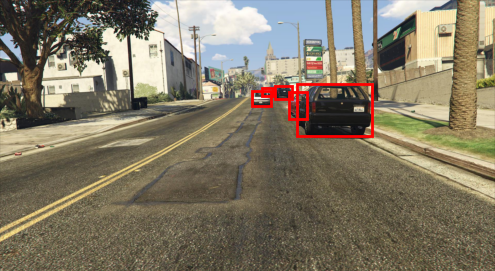
\includegraphics[width=.45\textwidth]{imgs/sim10korig.png}
                \hspace{.01\textwidth}
                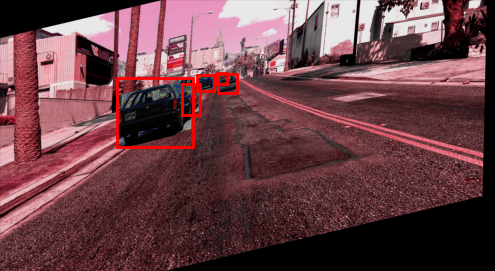
\includegraphics[width=.45\textwidth]{imgs/sim10kaug2.png}
            \end{center}
        }
        \item[\contour{DEgreen}{$\Rightarrow$}]<2-> \alert{\textbf{Domain randomization}}:
        \begin{itemize}
            \item Network is \quotes{overwhelmed} with widely different versions of the same training images
            \item Source data distribution may become closer to the target's
            \item No image from target domain is needed
        \end{itemize}
        \vspace*{5mm}
        \item<3-> Experiments confirm the hypothesis:
        \begin{itemize}
            \item Detection results are improved on \textit{RetinaNet} and \textit{Faster R-CNN}
            \item Color operators contribute the most
        \end{itemize}
    \end{itemize}
    \end{overlayarea}
\end{frame}

\begin{frame}[t]{Method}
    \framesubtitle{Adapting the Feature Pyramid Network}
    
    \begin{itemize}
        \item<1-> \alert{FPN}\footfullcite{lin2017feature} is widely used for object detection:
        \begin{itemize}
            \item Extract feature maps at multiple levels from a single image
            \item Sequence of convolutional layers, size divided by two at consecutive stages, with top-down connections
            \item Increases detection performances, but adversarial domain alignment is non-trivial
        \end{itemize}
        \only<1>{
            \begin{center}
                \item[]
                \fbox{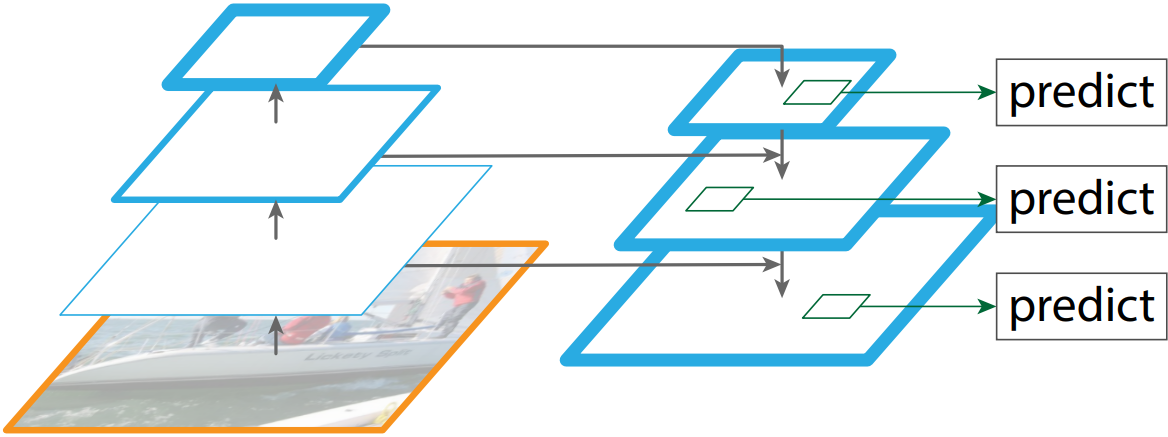
\includegraphics[width=.5\textwidth]{imgs/fpn.png}}
            \end{center}
        }
        \item<2-> Tested approaches:
        \begin{itemize}
            \item Align levels of extracted feature pyramid
            \item Align layers of the \alert{ResNet} feature extractor, input for FPN
        \end{itemize}
        \item<2-> Extracted representation is meaningful and independent of input domain
        \vspace*{5mm}
        \item<3-> Method is effective on \textit{RetinaNet}, but not on \textit{Faster R-CNN}
    \end{itemize}
\end{frame}

\begin{frame}{Method}
    \framesubtitle{Image statistics matching}
    \begin{itemize}
        \item Domain mapping approach that updates source image statistics to match the target domain\footfullcite{abramov2020simple}
        \vspace*{-4mm}
        \begin{center}
            \item[]
            \hspace{-.08\textwidth}
            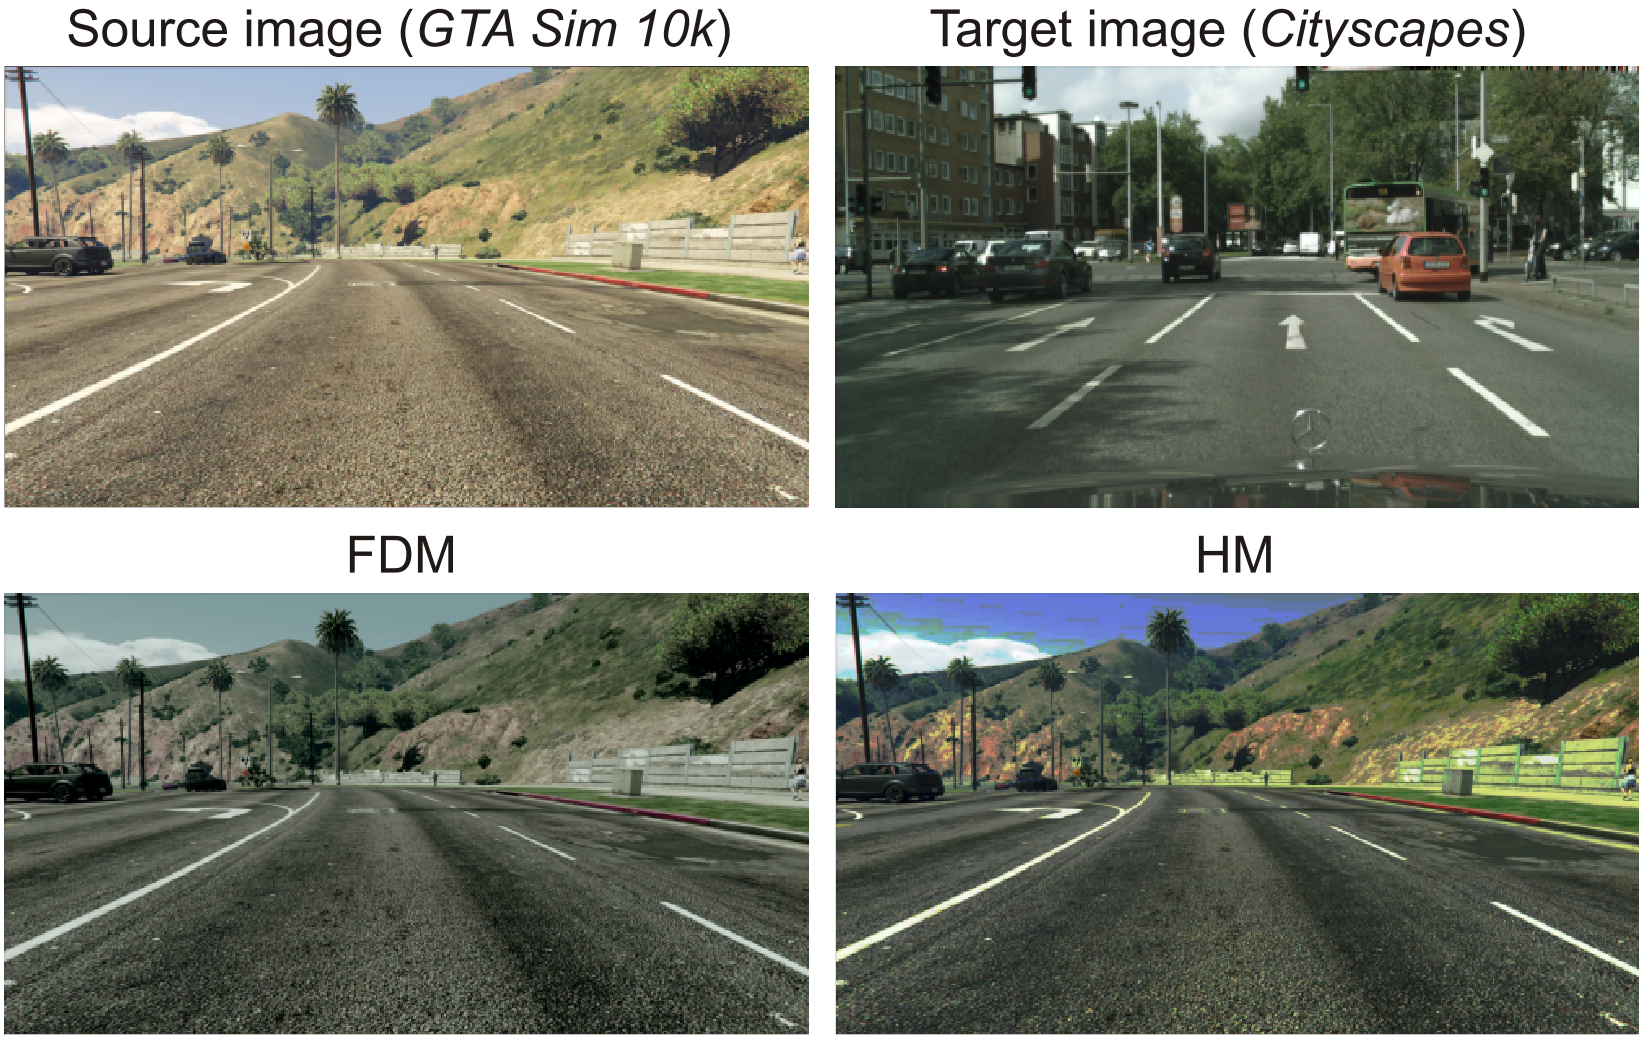
\includegraphics[width=.65\textwidth]{imgs/image26.png}
        \end{center}
    \end{itemize}
\end{frame}

\section{Results}

\begin{frame}{Results}
    \framesubtitle{Domain randomization}
    
    \begin{table}
        \centering
        \begin{NiceTabular}{|cccccc|cc|}
            \toprule
            \Block{1-6}{\scriptsize{\textbf{Transformations}}} & & & & & & \Block{1-2}{\scriptsize{\textbf{Detector}}} & \\
            \midrule
    		\Block{1-1}{\scriptsize{Horizon-}\\\scriptsize{tal flip}} & \Block{1-1}{\scriptsize{Rotation}} & \Block{1-1}{\scriptsize{Transla-}\\\scriptsize{tion}} & \Block{1-1}{\scriptsize{Color}\\\scriptsize{jitter}} & \Block{1-1}{\scriptsize{Solari-}\\\scriptsize{zation}} & \Block{1-1}{\scriptsize{Equali-}\\\scriptsize{zation}} & \Block{1-1}{\scriptsize{mAP@0.5}\\\scriptsize{RetinaNet}} & \Block{1-1}{\scriptsize{mAP@0.5}\\\scriptsize{Faster R-CNN}\\\scriptsize{w/ FPN}} \\
    		\midrule
    		$\checkmark$ & & & & & & 30.4 & 46.3  \\
    		$\checkmark$ & $\checkmark$ & $\checkmark$ & & & & 37.6 & 48.8  \\
    		$\checkmark$ & $\checkmark$ & $\checkmark$ & $\checkmark$ & & & 49.4 & \textbf{57.9}  \\
    		$\checkmark$ & $\checkmark$ & $\checkmark$ & $\checkmark$ & $\checkmark$ & $\checkmark$ & \textbf{52.7} & \textbf{57.9}  \\
    		\midrule
    		\Block[l]{1-6}{\scriptsize{Oracle}} & & & & & & 68.7 & 76.3 \\
    		\bottomrule
        \end{NiceTabular}
    \end{table}
    
    \begin{itemize}
        \item FPN drives \textit{Faster R-CNN} to better detection performances than \textit{RetinaNet}
    \end{itemize}
\end{frame}

\begin{frame}{Results}
    \framesubtitle{RetinaNet}
    
    \begin{table}
        \centering
        \begin{NiceTabularX}{\linewidth}{|X|cccc|c|}
            \toprule
            \Block[l]{2-1}{\scriptsize{\textbf{Method}}} & \Block{1-4}{\scriptsize{\textbf{Transformations}}} & & & & \Block{2-1}{\scriptsize{\textbf{mAP@0.5}}} \\
            \cmidrule{2-5}
            & \Block{1-1}{\scriptsize{Horizontal flip}} & \Block{1-1}{\scriptsize{Rotation}} & \Block{1-1}{\scriptsize{Translation}} & \Block{1-1}{\scriptsize{Color jitter}} & \\
            \midrule
            \scriptsize{Baseline} & $\checkmark$ & & & & 30.4 \\
            \midrule
            \Block[l]{3-1}{\scriptsize{Image statistics matching}} & $\checkmark$ & & & & 48.2   \\
            & $\checkmark$ & $\checkmark$ & $\checkmark$ & & 52.0 \\
            & $\checkmark$ & $\checkmark$ & $\checkmark$ & $\checkmark$ & \textbf{62.7} \\
            \midrule
            \Block[l]{3-1}{\scriptsize{Adversarial adaptation}} & $\checkmark$ & & & & 52.8   \\
            & $\checkmark$ & $\checkmark$ & $\checkmark$ & & 54.2 \\
            & $\checkmark$ & $\checkmark$ & $\checkmark$ & $\checkmark$ & 54.8 \\
            \midrule
            \scriptsize{Oracle} & $\checkmark$ & & & & 68.7 \\
    		\bottomrule
        \end{NiceTabularX}
    \end{table}
\end{frame}

\begin{frame}{Results}
    \framesubtitle{Faster R-CNN}
    
    \vspace*{-.5cm}
    \begin{table}
    	\centering
    	\begin{NiceTabularX}{\linewidth}{|X|c|cccc|c|}
    		\toprule
    		\Block[l]{2-1}{\scriptsize{\textbf{Method}}} & \Block{2-1}{\scriptsize{\textbf{FPN}}} & \Block{1-4}{\scriptsize{\textbf{Transformations}}} & & & & \Block{2-1}{\scriptsize{\textbf{mAP@0.5}}} \\
    		\cmidrule{3-6}
    		& & \Block{1-1}{\scriptsize{Horizontal flip}} & \Block{1-1}{\scriptsize{Rotation}} & \Block{1-1}{\scriptsize{Translation}} & \Block{1-1}{\scriptsize{Color jitter}} & \\
    		\midrule
    		\Block[l]{2-1}{\scriptsize{Baseline}} & & $\checkmark$ & & & & 33.7 \\
    		& $\checkmark$ & $\checkmark$ & & & & 46.3 \\
    		\midrule
    		\Block[l]{3-1}{\scriptsize{Image statistics matching}} & $\checkmark$ & $\checkmark$ & & & & 55.0   \\
    		& $\checkmark$ & $\checkmark$ & $\checkmark$ & $\checkmark$ & & 62.0 \\
    		& $\checkmark$ & $\checkmark$ & $\checkmark$ & $\checkmark$ & $\checkmark$ & \textbf{62.5} \\
    		\midrule
    		\Block[l]{3-1}{\scriptsize{Adversarial adaptation}} & & $\checkmark$ & & & & 36.3   \\
    		& \scriptsize{Aligned} & $\checkmark$ & & & & 45.0 \\
    		& \Block{1-1}{\scriptsize{ResNet}\\\scriptsize{aligned}} & $\checkmark$ & & & & 46.8 \\
    		\midrule
    		\scriptsize{Oracle} & $\checkmark$ & $\checkmark$ & & & & 76.3 \\
    		\bottomrule
    	\end{NiceTabularX}
    \end{table}
\end{frame}


\section{Conclusions}

\begin{frame}{Conclusions}
    \begin{itemize}
        \item<1-> Performance gap due to the domain shift between cheap synthetic images and expensive real images
        \vspace*{5mm}
        \con<2-> Popular methods for domain adaptive object detection depend on architecture-specific components
        \con<2-> Adversarial alignment may be unstable 
        \pro<2-> Domain mapping methods are effective with low training and implementation cost: suitable for production environments
        \vspace*{5mm}
        \item<3-> Domain randomization through data augmentation can be enough
        \item<3-> ...and can support more advanced domain adaptation methods
    \end{itemize}
\end{frame}


\usebeamertemplate{endpage}
\begin{frame}[plain]
    \begin{center}
        \color{white}
        \huge\bf Thank you for your attention!
    \end{center}
\end{frame}

\end{document}